%!TEX root = ../thesis.tex
%Adding the above line, with the name of your base .tex file (in this case "thesis.tex") will allow you to compile the whole thesis even when working inside one of the chapter tex files

\chapter{Data Analysis} \label{chap:4}

\section{The Measurement Equation}\label{sec:4.1}

Measurement Equation: Appendix CASA guides

\begin{figure}[hbt!]
\centering 
          \includegraphics[trim=0pt 0pt 0pt 0pt,clip,scale=0.5]{/home/eamon/thesis/thesis_template/4/cash_flow.ps}
\caption[]{}
\label{fig:4.1}
\end{figure}

Data analysis section from both papers

\section{Data Examination and Flagging}\label{sec:4.2}

\section{Calibration}\label{sec:4.3}

\section{Imaging}\label{sec:4.4}

CLEAN vs MEM vs Multi-scale Clean (for Peter!)

second sources (maps)

Dirty Image, PSF

Show images of calibrators